\documentclass[10pt]{article}
\usepackage[web]{../problem-collection}
\newcommand{\pp}[1]{REMOVE}
\newcommand{\p}[1]{REMOVE}

\begin{document}

\begin{titlepage}
    \centering
    \vspace{10cm}
    {\sffamily\Huge \mbox{200 EESTI FÜÜSIKAOLÜMPIAADI}\\ ÜLESANNET AASTATEST\\ 2018 -- 2025\par}
    \vspace{1cm}
    {\Large koos vihjete ja lahendustega\par}
    \vfill
    {\Large Koostas Taavet Kalda}

    \vfill

    % Bottom of the page
    {\large 2025}
\end{titlepage}

\raggedbottom % Because of twosided
\mbox{}\vfill

\textcopyright~Autoriõigused: Eesti Matemaatika Selts, Tallinna Tehnikaülikool,
Tartu Ülikool, ülesannete autorid ja Taavet Kalda.
\vspace{0.5\baselineskip}

Kogumiku koostamist toetasid: Eesti Matemaatika Seltsi fond ``Benoit Mandelbroti Jälgedes'', Robert Kitt ja Tallinna Tehnikaülikool.
\vspace{0.5\baselineskip}

\newpage

\tableofcontents
\newpage

{\setlength{\parindent}{24pt}
\section{Sissejuhatus}

Siia on koondatud 200 gümnaasiumi ülesannet Eesti füüsikaolümpiaadi piirkonnavoorudest, lõppvoorudest ja lahtistest võistlustest. Igale ülesandele on juurde kirjutatud paarilauseline vihje. Juhul kui õpilane jääb ülesannet lahendades toppama, on tal võimalik vihjet lugeda ning teisele katsele minna.

%Tegu on teise kogumikuga Eesti füüsikaolümpiaadi ülesannete kogude seeriast, kus esimene kattis 200 ülesannet ajavahemikust 2012---2018.

Ülesanded on jaotatud teemade kaupa ning teemasiseselt raskuse järgi. Raskustaset tähistatakse kuni viie tärniga. Ülesannete lihtsamaks otsimiseks on ülesannete numbrite ette pandud \enquote{Ü}, vihjete ette \enquote{V} ja lahenduste ette \enquote{L}. Näiteks ülesande 133 teksti number on kujul Ü133. Iga ülesande juures on kirjas ka selle autor ning olümpiaadi vooru lühinimetus, lisaks lühendid P 1, G 1 jne, kus tähed tähistavad põhikooli- ja gümnaasiumiastet. Näiteks G 9 viitab gümnaasiumiastme 9. ülesandele.

%Kogumiku koostamise käigus eemaldati erinevatel põhjustel 3 ülesannet.

Lisaks leiate kogumiku lõpust kogumiku poolt kaetud lahtiste ja lõppvoorude esimese ja teise järgu saanud õpilaste ning ülesannete autorite nimekirja.}
\newpage
\setlength{\parindent}{0pt}

        \section{Ülesanded}
        \toggleStatement
        \subsection{\protect\StrSubstitute{Kinemaatika}{-}{ }}

\graphicspath{{../probs_b3/}}

% Ü1
\setAuthor{Markus Rene Pae}
\setRound{lahtine}
\setYear{2019}
\setNumber{G 1}
\setDifficulty{1}
\setTopic{Kinemaatika}

\prob{Ristmik}
Juku, sõites autoga ($v = \SI{90}{\kilo\meter\per\hour}$), läheneb Y-kujulisele ristmikule. Kui tal on ristmikuni jäänud veel $l = \SI{150}{\meter}$ märkab Juku, et kõrvalharu pealt sõidab ristmiku poole ka teine auto, mille ristmikuni jäänud vahemaa ja kiiruse projektsioonid Juku sõidusuunale on võrdsed Juku auto omadega. Kokkupõrke vältimiseks kiirendab Juku kiirendusega $a = \SI{0.5}{\meter\per\second\squared}$. Mis on autode vahemaa, kui teine auto jõuab ristmikuni? Teede vaheline nurk on \ang{15}.
\probend
\bigskip
\newpage\subsection{\protect\StrSubstitute{Varia}{-}{ }}

% Ü2
\setAuthor{Valter Kiisk}
\setRound{lahtine}
\setYear{2019}
\setNumber{G 2}
\setDifficulty{2}
\setTopic{Varia}

\prob{Pumpjaam}
\begin{wrapfigure}[9]{r}{0.45\linewidth}
    \vspace{-10pt}
	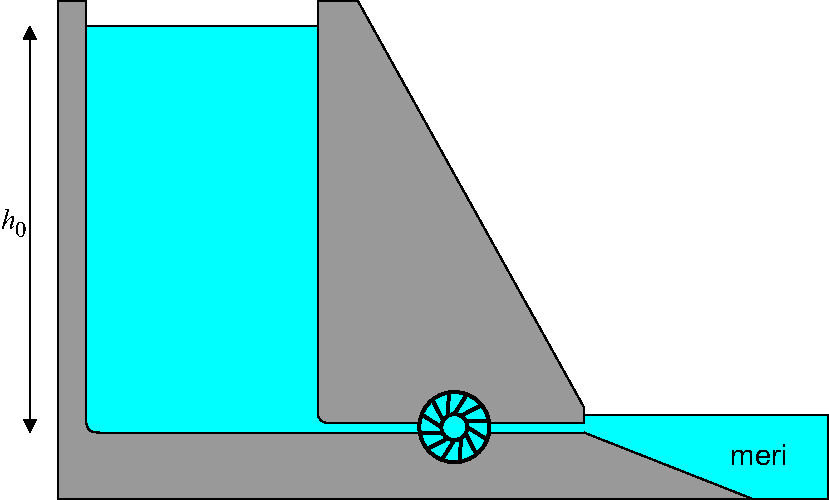
\includegraphics[width=\linewidth]{2019-lahg-02-yl.pdf}
\end{wrapfigure}

Arenenud riikides on elektrienergia tarbimine, võrrelduna riigi pindalaga, suurusjärgus \SI{100}{\kilo\watt\per\kilo\meter\squared}. Joonisel on kujutatud teatava pump-hüdroakumulatsiooni elektrijaama skeem. Eeldame, et alumiseks reservuaariks on meri (mille tase püsib praktiliselt muutumatu) ja ülemise reservuaari põhi ulatub merepinna tasemeni. Elektrienergia ületootmise ajal pumbatakse merevett ülemisse reservuaari kuni kõrguseni $h_0=\SI{100}{m}$. Energiadefitsiidi ajal toimib sama süsteem hüdroelektrijaamana. Ignoreerides energia konverteerimis- ja ülekandekadusid, kui suure osa riigi pindalast peaks sellised pumpjaamad (st ülemise reservuaari pindala) moodustama, et muude elektritootjate äralangemisel kindlustada elektrienergia varu 24 tunniks? Vee tihedus on $\rho=\SI{1000}{kg/m^3}$ ja raskuskiirendus $g=\SI{9.8}{m/s^2}$.
\probend
\bigskip
\newpage\subsection{\protect\StrSubstitute{Optika}{-}{ }}

% Ü3
\setAuthor{Hans Daniel Kaimre}
\setRound{lahtine}
\setYear{2019}
\setNumber{G 3}
\setDifficulty{2}
\setTopic{Optika}

\prob{Lääts}
Optiline süsteem koosneb punktvalgusallikast ja ekraanist, mille vahele on asetatud õhuke koondav lääts. Ekraani ja valgusallika vaheline kaugus on $L$ ning läätse asukohta saab vabalt liigutada. Millist tingimust peab rahuldama läätse fookuskaugus selleks, et ekraanile oleks võimalik tekitada tõelist kujutist? Missugune on optilise süsteemi suurendus juhul kui läätse fookuskaugus on võimalikult suur?
\probend
\bigskip
\newpage\subsection{\protect\StrSubstitute{Elektrostaatika}{-}{ }}

% Ü4
\setAuthor{Kaarel Hänni}
\setRound{lahtine}
\setYear{2019}
\setNumber{G 4}
\setDifficulty{4}
\setTopic{Elektrostaatika}

\prob{Laetud tasand}
Ruumis on ühtlaselt laetud tasand ja paaritu arv võrdseid laenguid, mis ei asu tasandil. Tõesta, et tasandile mõjuv resultantjõud ei saa olla 0.
\probend
\bigskip
\newpage\subsection{\protect\StrSubstitute{Dünaamika}{-}{ }}

% Ü5
\setAuthor{Erkki Tempel}
\setRound{lahtine}
\setYear{2019}
\setNumber{G 5}
\setDifficulty{4}
\setTopic{Dünaamika}

\prob{Kuulid}
Mängupüssist lastakse otse üles kummist kuul algkiirusega $v$. Sel ajal, kui esimene kuul on õhus, lastakse aja $t$ pärast üles teine samasugune kuul samuti algkiirusega $v$. Kui kõrgele $h$ põrkab esimene kuul pärast esimest elastset põrget?
\probend
\bigskip
\newpage\subsection{\protect\StrSubstitute{TODO}{-}{ }}

% Ü6
\setAuthor{Ardi Loot}
\setRound{lahtine}
\setYear{2019}
\setNumber{G 6}
\setDifficulty{6}
\setTopic{TODO}

\prob{LED}
LED-lamp koosneb $N=10$-st valgusdioodist ning mida toidetakse vaheduvvooluga sagedusega $f=\SI{50}{Hz}$ ning maksimaalse pingega $U=\SI{320}{V}$ läbi takisti $R=\SI{400}{\ohm}$, kondensaatori ning alaldi

LED-lamp koosneb $N=10$-st valgusdioodist (nimipinge $U_{D}=\SI{3.0}{V}$ ja -vool $I_{D}=\SI{100}{mA}$), mida toidetakse vahelduvvooluga (pinge maksimumväärtus $U=\SI{320}{V}$ ja sagedus $f=\SI{50}{Hz}$) läbi takisti ($R=\SI{400}{\ohm}$), kondensaatori ja alaldi (lugeda ideaalseks). Kui suur peab olema kondensaatori mahtuvus $C,$ et valgusdioodid põleksid võimalikult heledalt, kuid ei põleks läbi?

\emph{Märkus:} Takisti ja kondensaatori näivtakistus on $Z=\sqrt{R^{2}+X_{C}^{2}}$, kus $X_{C}=1/\left(2\pi fC\right)$ ning võib eeldada sinusoidaalset voolu ja pinget aladi ees.
\begin{center}
	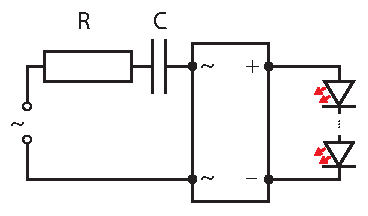
\includegraphics[width=0.6\linewidth]{2019-lahg-06-yl.pdf}
\end{center}
\probend
\bigskip

% Ü7
\setAuthor{Jaan Kalda}
\setRound{lahtine}
\setYear{2019}
\setNumber{G 7}
\setDifficulty{7}
\setTopic{Kinemaatika}

\prob{Külm gaas}
\begin{wrapfigure}[8]{r}{0.3\textwidth}
	\vspace{-5pt}
	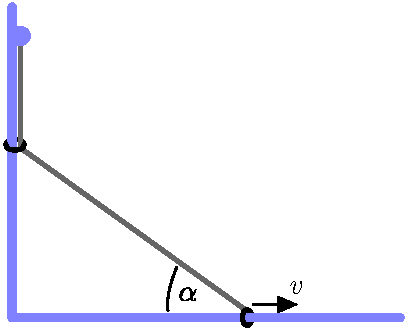
\includegraphics[width=0.3\textwidth]{2019-lahg-07-yl.pdf}
\end{wrapfigure}

Niit kogupikkusega $L$ on kinnitatud kahest üksteisega ristuvast lõigust koosneva relsi külge nii, nagu näidatud joonisel: üks niidi ots on fikseeritud jäigalt vertikaalse relsiosa külge kaugusele $h$ relsi nurgast, seejärel läheb niit läbi tillukese rõnga, mis saab libiseda mööda vertikaalset relssi ning niidi teine ots on kinnitatud tillukese rõnga kaudu horisontaalse relsi külge. Alumist rõngast hakatakse liigutatama konstantse kiirusega $v$. Leida teise rõnga kiirus ja kiirendus hetkel, mil nöör moodustab nurga $\alpha$ horisontaalsihiga.
\probend
\bigskip
\newpage\subsection{\protect\StrSubstitute{Termodünaamika}{-}{ }}

% Ü8
\setAuthor{Jaan Kalda}
\setRound{lahtine}
\setYear{2019}
\setNumber{G 8}
\setDifficulty{8}
\setTopic{Termodünaamika}

\prob{Külm gaas}
Tihedalt suletud anumas on monomolekulaarne gaas molaarmassiga $\mu$ ja tihedusega $\rho$ temperatuuril $T_0$. Anum on silindriline ja tema telg vertikaalne. Anum liigub ülevalt alla algkiirusega $v$ ja peatub hetkeliselt; eeldada, et $v\gg \sqrt{RT_0/\mu}$, $R$ tähistab universaalset gaasikonstanti. Millist rõhku avaldab gaas anuma põhjale\\
\osa vahetult peale anuma seinte peatumist;\\
\osa peale seda, kui gaas jõuab termodünaamilisse tasakaalu. Gaasi soojusvahetust anuma seintega ignoreerida, eeldada, et põrkumisel seintega on molekulide eemaldumisnurk pinnanormaali suhtes võrdne langemisnurgaga.
\probend
\bigskip
\newpage\subsection{\protect\StrSubstitute{Magnetism}{-}{ }}

% Ü9
\setAuthor{Jaan Kalda}
\setRound{lahtine}
\setYear{2019}
\setNumber{G 9}
\setDifficulty{9}
\setTopic{Magnetism}

\prob{Hantel}
Kaks metallkera raadiusega $R$ ja massiga $m$ on ühendatud koaksiaalselt metallvardaga, mille pikkus $L$ on hulga suurem $R$-st ja mille mass ning diameeter on tühiselt väiksed. Kogu süsteem asub kaalutuse tingimustes teljega ristsihilises homogeenses magnetväljas induktsiooniga $B$. Ühele kuulikestest kantakse hetkeliselt elektrilaeng $Q$; visandage ühel ja samal joonisel mõlema kuulikese trajektoorid edasise liikumise käigus. Eeldada, et varda elektriline takistus on tühiselt väike ja et $\varepsilon_0B^2L^2R\ll m$, kus $\varepsilon_0$ tähistab vaakumi dielektrilist läbitavust.
\probend
\bigskip

% Ü10
\setAuthor{Andres Põldaru}
\setRound{lahtine}
\setYear{2019}
\setNumber{G 10}
\setDifficulty{10}
\setTopic{Varia}

\prob{Lame maa}
Juku lendab lennukiga $h=\SI{10}{km}$ kõrgusel, suunab kaamera optilise peatelje horisondile ja teeb pildi. Seejärel trükib ta pildi $10\times \SI{10}{cm}$ paberile ($L=\SI{10}{cm}$). Kui palju on pildi servas horisont maakera kumeruse tõttu madalamal kui pildi keskel? Võib eeldada, et see suurus on väga väike. Kaamera vaatenurk $2\beta=\SI{50}{\degree}$, Maa raadius $R=\SI{6000}{km}$.
\probend
\bigskip
\newpage\normalsize\section{Vihjed}
        \toggleHint
        
% V1
\setAuthor{Markus Rene Pae}
\setRound{lahtine}
\setYear{2019}
\setNumber{G 1}
\setDifficulty{1}
\setTopic{Kinemaatika}

\prob{Ristmik}
\hint
Kõigepealt tuleb leida kui palju kulub Jukul kiirendamata aega ristmikuni jõudmiseks, sest see ühtib ajaga, millega teine auto ristmikuni jõuab.
\probend
\bigskip

% V2
\setAuthor{Valter Kiisk}
\setRound{lahtine}
\setYear{2019}
\setNumber{G 2}
\setDifficulty{2}
\setTopic{Varia}

\prob{Pumpjaam}
\hint
Ülesande lahendamise käigus on mugav kasutada reservuaari pindala $S$, vaatamata sellele, et see pärast välja taandub. Lisaks tasub mõelda, mis on reservuaari massikeskme kõrgus.
\probend
\bigskip

% V3
\setAuthor{Hans Daniel Kaimre}
\setRound{lahtine}
\setYear{2019}
\setNumber{G 3}
\setDifficulty{2}
\setTopic{Optika}

\prob{Lääts}
\hint
Tõelise kujutise tekkimise tingimuse saab kirja panna läätse valemi kaudu funktsioonina läätse kaugusest ekraanist ja fookuskaugusest.
\probend
\bigskip

% V4
\setAuthor{Kaarel Hänni}
\setRound{lahtine}
\setYear{2019}
\setNumber{G 4}
\setDifficulty{4}
\setTopic{Elektrostaatika}

\prob{Laetud tasand}
\hint
Ühe laengu poolt tasandile avaldatav jõud on Newtoni kolmanda seaduse kohaselt võrdne ja vastasmärgiline tasandi poolt laengule avaldatava jõuga.
\probend
\bigskip

% V5
\setAuthor{Erkki Tempel}
\setRound{lahtine}
\setYear{2019}
\setNumber{G 5}
\setDifficulty{4}
\setTopic{Dünaamika}

\prob{Kuulid}
\hint
Ülesande lahendus lihtsustub oluliselt täheldades, et vahetult enne kokkupõrget on kuulide kiirused võrdsed, aga vastassuunalised.
\probend
\bigskip

% V6
\setAuthor{Ardi Loot}
\setRound{lahtine}
\setYear{2019}
\setNumber{G 6}
\setDifficulty{6}
\setTopic{TODO}

\prob{LED}
\hint

\probend
\bigskip

% V7
\setAuthor{Jaan Kalda}
\setRound{lahtine}
\setYear{2019}
\setNumber{G 7}
\setDifficulty{7}
\setTopic{Kinemaatika}

\prob{Külm gaas}
\hint
Üks lähenemisviisidest on tähistada alumise ja ülemise rõngaste kaugused nurgast vastavalt kui $x$ ja $y$. Sellisel juhul on $x$ ajaline tuletis $v$ ning otsitavad suurused on $y$ esimene ja teine ajaline tuletis.
\probend
\bigskip

% V8
\setAuthor{Jaan Kalda}
\setRound{lahtine}
\setYear{2019}
\setNumber{G 8}
\setDifficulty{8}
\setTopic{Termodünaamika}

\prob{Külm gaas}
\hint
Esimese osa jaoks tasub vaadelda kui palju annavad molekulid väikse ajavahemiku $t$ jooksul anuma alumisele seinale impulssi üle. Teise osa jaoks kehtib energia jäävuse seadus.
\probend
\bigskip

% V9
\setAuthor{Jaan Kalda}
\setRound{lahtine}
\setYear{2019}
\setNumber{G 9}
\setDifficulty{9}
\setTopic{Magnetism}

\prob{Hantel}
\hint
Kriitiline tähelepanek on, et hantel kujuneb ekvipotentsiaalseks, st laengud korraldavad üksteist ümber nõnda, et see tingimus kehtiks.
\probend
\bigskip

% V10
\setAuthor{Andres Põldaru}
\setRound{lahtine}
\setYear{2019}
\setNumber{G 10}
\setDifficulty{10}
\setTopic{Varia}

\prob{Lame maa}
\hint
Lahendamise käigus saab teha paar lihtsustavat lähendust. Esiteks moodustab maakera horison kaamerale ringjoone ning teiseks on kõik Maa horisondi punktid efektiivselt lõpmatuses ning kaamera poolt samaaegselt fokusseeritud. Seega võib kõik kiired projitseerida vabalt valitud tasandisse, mis on kaamera optilise peateljega risti. Kuna meid huvitab kaamera pildi peal horisondi kõrguse muutus vertikaalteljes, siis tasub ülesande geomeetriat ka selles teljestikus vaadelda.
\probend
\bigskip
\newpage\section{Lahendused}
        \toggleSolution
        
% L1
\setAuthor{Markus Rene Pae}
\setRound{lahtine}
\setYear{2019}
\setNumber{G 1}
\setDifficulty{1}
\setTopic{Kinemaatika}

\prob{Ristmik}
\solu
Kui Juku ja teise auto projitseeritud kaugus ristmikust ja kiirused on samad, siis nad jõuavad ristmikule täpselt sama ajaga
\[
t = s/v = \frac{\SI{150}{\meter}}{\SI{90}{\kilo\meter\per\hour}} = \frac{\SI{150}{\meter}}{\SI{25}{\meter\per\second}} = \SI{6}{\second}.
\]
Kui Juku saavutaks hetkeliselt kiirenduse $a = \SI{0.5}{\meter\per\second\squared}$, siis selle ajaga jõuaks ta läbida
\[
s = v_0 t + a t^2/2 = \SI{159}{\meter}.
\]
Seega on teise auto ristmikule jõudes autode vahemaa $\SI{9}{\meter}$. Nurk ei oma antud ülesandes tähtsust.
\probend
\bigskip

% L2
\setAuthor{Valter Kiisk}
\setRound{lahtine}
\setYear{2019}
\setNumber{G 2}
\setDifficulty{2}
\setTopic{Varia}

\prob{Pumpjaam}
\solu
Olgu reservuaari pindala $S$. Vee mass on $m=\rho V=\rho h_0S$. Selle massikese on tõstetud kõrgusele $h=h_0/2$, seega potentsiaalne energia on $mgh=\frac{1}{2}\rho gh_0^2S$ ja energia pinnaühiku kohta
\[
w_s=\frac{1}{2}\rho gh_0^2\approx \SI{49}{\mega\joule\per\meter\squared}\approx\SI{13.6}{kWh\per\meter\squared}.
\]
Energiavajaduse rahuldamiseks on vaja keskmist energiatihedust
\[
w_t=\SI{100}{\kilo\watt\per\kilo\meter\squared}\cdot \SI{24}{\hour}=\SI{2400}{kWh\per\kilo\meter\squared}=\SI{0.0024}{kWh\per\meter\squared}.
\]
Otsitav suurus on seega $w_t/w_s\approx \num{1.8e-4}$.
\probend
\bigskip

% L3
\setAuthor{Hans Daniel Kaimre}
\setRound{lahtine}
\setYear{2019}
\setNumber{G 3}
\setDifficulty{2}
\setTopic{Optika}

\prob{Lääts}
\solu
Otsime kaugust $s$, mille korral tekib ekraanile reaalne kujutis, paneme kirja süsteemi jaoks läätse valemi:
$$
\frac{1}{s}+\frac{1}{L-s}=\frac{1}{f}\Rightarrow \frac{L}{s(L-s)}=\frac{1}{f} \Rightarrow s^2-LS+Lf=0.
$$
Tegu on tavalise ruutvõrrandiga, kust saame, et
$$
s_{1,2}=\frac{1}{2}\left(L\pm\sqrt{L(L-4f)}\right).
$$
Kuna $s$ on reaalne suurus, mitte imaginaarne, siis $L-4f \geq 0$, kust omakorda saame $f$ tingimuseks, et $f \leq L/4$. Seega kõige suurem võimalik fookuskaugus on $f = L/4$, mille korral saame $s_{1,2} = L/2$ ja suurenduse $M=s_2/s_1 = 1$ ehk kujutis on sama suur kui kujutist tekitav objekt.
\probend
\bigskip

% L4
\setAuthor{Kaarel Hänni}
\setRound{lahtine}
\setYear{2019}
\setNumber{G 4}
\setDifficulty{4}
\setTopic{Elektrostaatika}

\prob{Laetud tasand}
\solu
Ühe laengu poolt tasandile avaldatav jõud on Newtoni kolmanda seaduse kohaselt võrdne ja vastasmärgiline tasandi poolt laengule avaldatava jõuga. Seega on tasandile kokku mõjuv jõud 0 siis ja ainult siis, kui tasandi poolt laengutele avaldatud jõudude summa on 0. Tasandi elektriväli on konstantne ja risti tasandiga (ja tasandi eri pooltel erisuunaline). Seega on tasandi poolt laengutele avaldatud jõudude summa 0 siis ja ainult siis, kui kummalgi pool tasandit on võrdne arv laenguid. Laenguid on kokku paaritu arv, seega see on võimatu.
\probend
\bigskip

% L5
\setAuthor{Erkki Tempel}
\setRound{lahtine}
\setYear{2019}
\setNumber{G 5}
\setDifficulty{4}
\setTopic{Dünaamika}

\prob{Kuulid}
\solu
Kuna kuulid lastakse välja sama algkiirusel ning kokkupõrge toimub ühel kõrgusel, siis energia jäävuse põhjal on vahetult enne kokkupõrget kuulide kiirused samad, kuigi vastassuunalised. Kui põrkuvad kokku kaks ühesugust kuuli samade kiirustega, siis energia ja impulsi jäävuse tõttu on peale kokkupõrget nende kiirused samad, mis enne, kuid vastupidise märgiga. Seetõttu saavutab esimene kuul jälle oma esialgse maksimaalse kõrguse, mis on energia jäävuse seadusest leitav kui $h=v^2/2g$.

%\textbf{Alternatiivne lahendus:} 
%Esimese kuuli kõrgus on \(h_1(t_0) = vt_0 - gt_0^2/2\) ja teise kuuli kõrgus \(h_2(t_0) = v(t_0-t) - g(t_0 - t)^2/2\), kui esimene kuul lastakse õhku, siis \(t_0 = 0\). Põrke hetkel on kuulide kõrgused võrdsed. Sellest saame avaldada põrkehetke \(t_0 = t_p\).
%\begin{align*}
%    vt_p - gt_p^2/2 &= v(t_p-t) - g(t_p -t)^2/2, \\
%    vt_p - gt_p^2/2 &= vt_p - vt - gt_p^2/2 + 2gtt_p/2 - gt^2/2,\\
%    gtt_p &= vt + gt^2/2, \\
%    t_p &= v/g + t/2.
%\end{align*}
%Seda aega kasutades saame leida kummagi kuuli kiirused põrke hetkel. \(v_1 = v - gt_p = v - v - gt/2 = -gt/2\) ja \(v_2 = v -gt(t_p-t) = gt/2\) ehk \(v_p = |v_1| = |v_2|\). Seda saab ka tuletada energiajäävusest, et samal kõrgusel on kuulide kiiruste absoluutväärtused võrdsed. Elastse põrke korral kehtib nii impulsi kui ka energia jäävust, millest tuleneb, et võrdsete masside korral kuulide kiirused vahetuvad, ehk võrdsete vastassuunaliste kiiruste korral kiiruste suunad vahetuvad ja esimene kuul põrkab otse üles tagasi. Leiame kõrguse, kus toimus põrge
%\[h_p = vt_p - gt_p^2/2 = v^2/g + vt/2 - g(v^2/g^2 + vt/g + t^2/4)/2 = v^2/2g - gt^2/8.\]
%Pärast põrget tõusis esimene kuul veel kõrguse \(h_+ = v_p^2/2g = (gt/2)^2/2g = gt^2/8.\) Seega kuuli maksimaalne kõrgus pärast esimest põrget on \(h_p + h_+ = v^2/2g,\) mis oli ka esimese kuuli maksimaalne kõrgus enne põrget.
\probend
\bigskip

% L6
\setAuthor{Ardi Loot}
\setRound{lahtine}
\setYear{2019}
\setNumber{G 6}
\setDifficulty{6}
\setTopic{TODO}

\prob{LED}
\solu
Valgusdioodid põlevad võimalikult heledalt, ja ei põle läbi, nimipingel
ja voolul. Pinge jaotumise kohta saab kirja panna võrrandi $U=I_{D}Z+NU_{D}$
ja seda lahendades leida vajaliku takisti ja kondensaatori näivtakistuse 
\begin{equation*}
Z=\frac{U-NU_{D}}{I_{D}}=\SI{2.9}{k\Omega}.
\end{equation*}
Kasutades takisti ja kondensaatori näivtakistuse valemit saame avaldada
vajaliku mahtuvuse
\begin{equation*}
C=\frac{1}{2\pi f\sqrt{Z^{2}-R^{2}}}\approx\SI{1.1}{\mu F}.
\end{equation*}
\probend
\bigskip

% L7
\setAuthor{Jaan Kalda}
\setRound{lahtine}
\setYear{2019}
\setNumber{G 7}
\setDifficulty{7}
\setTopic{Kinemaatika}

\prob{Külm gaas}
\solu
Alghetkel on molekulide vertikaalkiirus soojuskiirusest palju suurem. Molekulid lähenevad põhjale kiirusega $v$, seega lühikese ajavahemiku $t$ jooksul jõuavad põhjaga põrkuda molekulid ruumalast $vtS$, kus $S$ on põhja pindala, kogumassiga $\rho vtS$. Peale põrkumist lahkuvad nad kiirusega $v$, seetõttu said nad põhjalt koguimpulsi $\Delta p=2\rho v^2tS$. See vastab jõule $F=\Delta p/t$ ja rõhule $p=F/S=2\rho v^2$.

Pikema aja möödudes saavutavad molekulid soojusliku tasakaalu, st nende kiirusjaotus muutub isotroopseks ja algne kineetiline koguenergia muutub siseenergiaks: $U=V\rho v^2/2$, kus $V$ tähistab anuma ruumala. Teisest küljest,
\[
U=\frac 32 \frac{\rho V}\mu RT,
\]
millest $v^2=3 RT/\mu$ ning $p=\rho RT/\mu=\rho v^2/3$.
\probend
\bigskip

% L8
\setAuthor{Jaan Kalda}
\setRound{lahtine}
\setYear{2019}
\setNumber{G 8}
\setDifficulty{8}
\setTopic{Termodünaamika}

\prob{Külm gaas}
\solu
Alghetkel lähenevad põhjale molekulid kiirusega $v$, seega lühikese ajavahemiku $t$ jooksul jõuavad põhjaga põrkuda molekulid ruumalast $vtS$, kus $S$ on põhja pindala, kogumassiga $\rho vtS$. Peale põrkumist lahkuvad nad kiirusega $v$ seetõttu said nad põhjalt koguimpulsi $\Delta p=2\rho vtS$. See vastab jõule $F=\Delta p/S$ ja rõhule $p=F/S=2\rho v$.

Pikema aja möödudes saavutavad molekulid soojusliku tasakaalu, st nende kiirusjaotus muutub isotroopseks ja algne kineetiline koguenergia muutub siseenergiaks: $U=V\rho v^2/2$, kus $V$ tähistab anuma ruumala. Teisest küljest, $U=\frac 32 \frac{\rho V}\mu RT$, millest $v^2=3 \frac{ RT}\mu$ ning $p=\frac{\rho}\mu RT=\rho v^2/3$.
\probend
\bigskip

% L9
\setAuthor{Jaan Kalda}
\setRound{lahtine}
\setYear{2019}
\setNumber{G 9}
\setDifficulty{9}
\setTopic{Magnetism}

\prob{Hantel}
\solu
Tagamaks, et hantel on ekvipotentsiaalne, voolab pool laengust teisele kerale; see toimub väga kiiresti, sest varda takistus on tühiselt väike (eeldame, et $RC$-aeg on hulga väiksem tsüklotronperioodist). Laengu voolamise ajal mõjub vardale Ampère'i jõud $F=BL\dv*{q}{t}$, kus $q$ tähistab teise kera laengut. Seetõttu on ülekantav jõuimpulss leitav kui $\Delta p=\int F\mathrm dt=\int BL\mathrm dq = BLQ/2$. Järelikult hakkab hantel liikuma kiirusega $v=\Delta p/2m=BLQ/4m$. Kuivõrd mõlema kuuli massid ja laengud on samad, siis hakkavad nad liikuma magnetväljas ühtmoodi, tsüklotronsagedusega $\omega=BQ/2m$ ja tsüklotronraadiusega $r=v/\omega=L/2$. Järelikult on kuulikeste trajektoorid ringjooned raadiusega $L/2$ ja diameetriga $L$, st tegemist on kahe üksteist puudutava ringjoonega.
\probend
\bigskip

% L10
\setAuthor{Andres Põldaru}
\setRound{lahtine}
\setYear{2019}
\setNumber{G 10}
\setDifficulty{10}
\setTopic{Varia}

\prob{Lame maa}
\solu
Lennukist nähtav maakera horisont moodustab ringjoone. Selle ringjoone eri punktid asuvad kaamerast eri kaugustel. Millise kujutise kaamera sensorile tekitab ringjoon, mille erinevate punktide kaugused kaamerast on erinevad?

Kõik kaamera vaatenurgas olevad ringjoone punktid on kaamerast väga kaugel. Kindlasti on lennukist näha kilomeetrite kaugusele, aga kaamera ise on väike. Seega on kõik horisondi punktid sisuliselt lõpmatuses ja võime heas lähenduses eeldada, et kaamera on nendele samaaegselt fokusseeritud. Kujutise leidmiseks tuleb kõik kiired projekteerida suvalisse tasandisse, mis on kaamera optilise peateljega risti.

Teeme joonise nr 1 maakera läbilõikega, kus Juku asub maakera kohal punktis $P$. Kaamera optiline peatelg on suunatud punkti $Q$. Olgu äärmine nähtav horisondi punkt $A$ ja selle projektsioon joonise tasandile $E$. Lennukist nähtava horisondi poolt moodustatud ringjoone keskpunkt on $O$. Projekteerime lennukist (punktist $P$) tõmmatud kiired tasandile, mis on optilise peateljega risti ja läbib punkti $E$.

Joonisel nr 2 on kujutatud horisondi ringjoont keskpunktiga $O$ eraldi, kus on näha äärmine nähtav punkt $A$ ja selle projektsioon $E$ eelmise joonise tasandisse. Heas lähenduses $\angle AOQ = \beta$, sest punktid $O$ ja $P$ on teineteisele lähedal ja pildi peal on punkti $A$ näha pildi servas peaaegu serva keskel (joonis 3). Täpselt pildi keskel on äärmiste punktide vahel $2\beta = \SI{60}{\degree}$.

\begin{center}
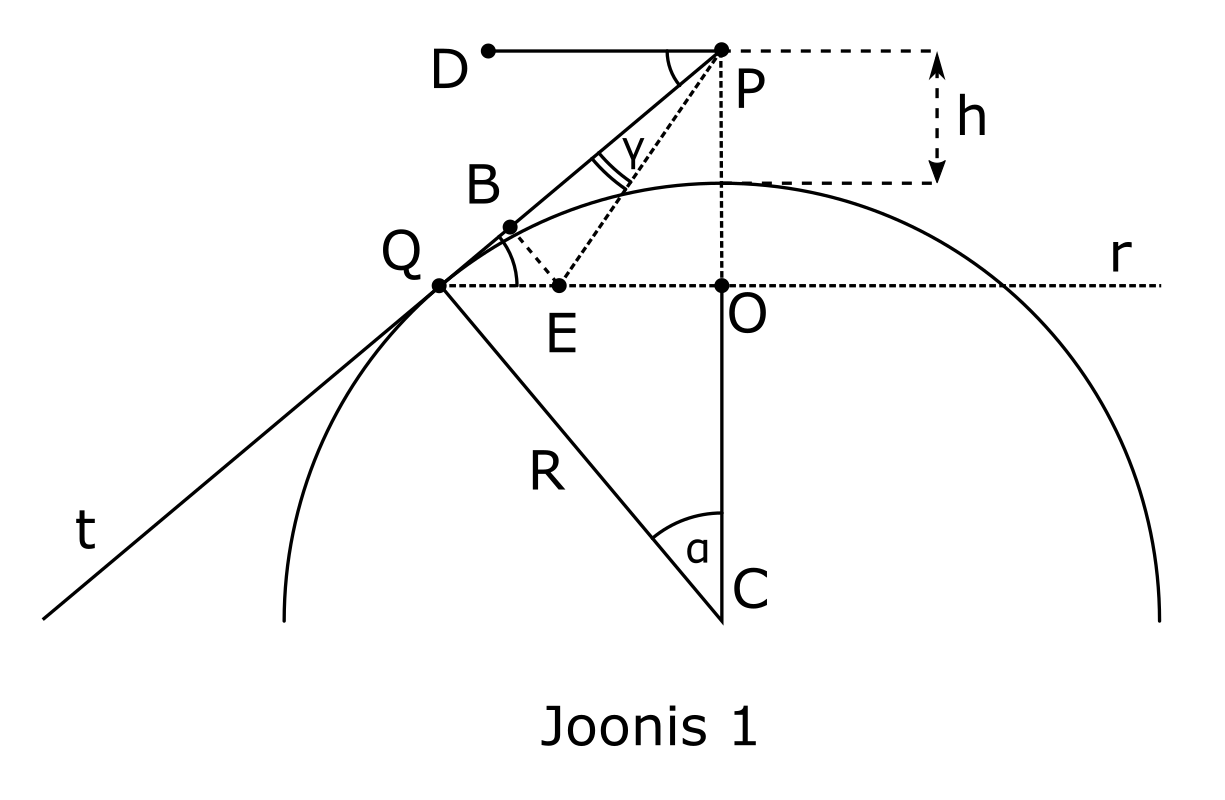
\includegraphics[width=0.50\textwidth]{2019-lahg-10-sol1.png}
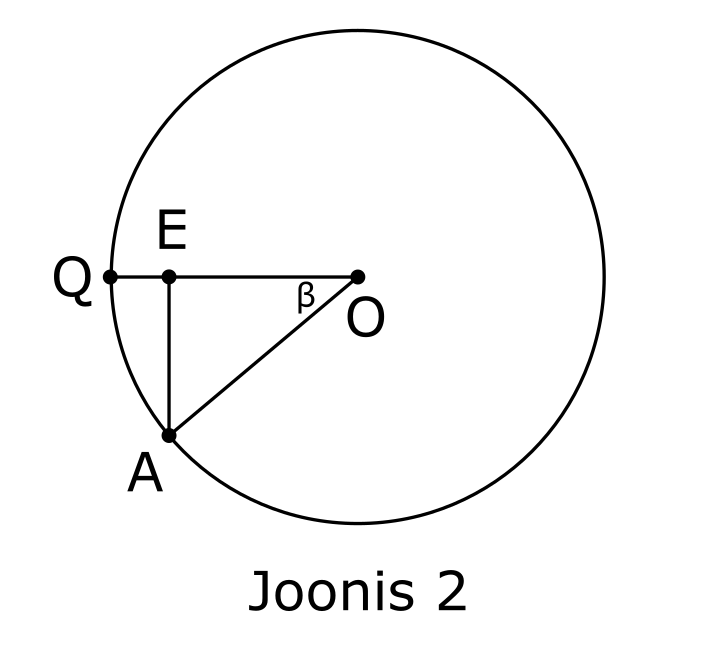
\includegraphics[width=0.265\textwidth]{2019-lahg-10-sol2.png}
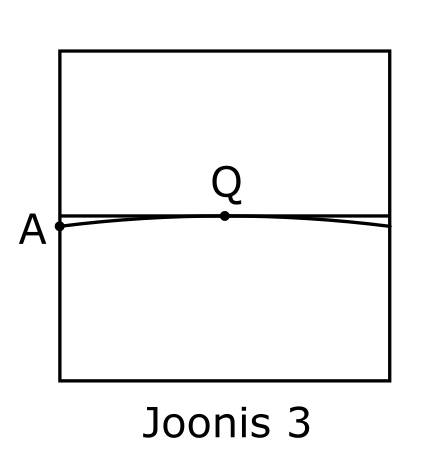
\includegraphics[width=0.215\textwidth]{2019-lahg-10-sol3.png}
\end{center}

Äärmise kiire projektsioon $|BE|$ vastab pildi peal üles-alla suunale. Seda projektsiooni iseloomustab nurk $\gamma=\SI{90}{\degree}-\alpha -\angle EPO$. 
Joonisel 1 leiame $$\cos{\alpha}=\frac{R}{R+h},$$ kust $$\alpha\approx\SI{3.3}{\degree}.$$ Veel leiame $$|OQ|=R\sin{\alpha}\approx \alpha R$$ ja
\[
|OP|=R+h-R\cos{\alpha}=\frac{(R+h)^2 - R^2}{R+h}\approx 2h.
\]
Joonise 2 abil leiame $$|OE|=|OQ|\cos{\beta}\approx \alpha R\cos{\beta}.$$

Nüüd saame leida joonisel 1 nurga $\gamma$.
$$\gamma = \SI{90}{\degree}-\alpha-\angle EPO = \SI{90}{\degree}-\alpha-\arctan{\frac{|OE|}{|OP|}}\approx \SI{0.34}{\degree}.$$
Nurgale vastava suuruse pildil saame leida, arvestades, et poolele vaatenurgale $\beta=\SI{25}{\degree}$ vastab $\SI{5}{cm}$. Projektsioonid samasse optilise peateljega ristuvasse tasandisse on võrdelised vastavate projektsioonidega välja prinditud pildil. $$\frac{x}{\SI{5}{cm}}=\frac{\tan{\gamma}}{\tan{\beta}} \rightarrow x = \SI{0.64}{mm}.$$

\textbf{Alternatiivne lahendus:}

Joonistame vaatluspunktist $P$ maakerale $M$ puutujakoonuse $K$ ning olgu $M$ ja $K$ puutejoon ring $R$ keskpunktiga $O$. Olgu ringil $R$ punkt $Q$ pildivälja keskpunktiks. Tähistame punkti $Q$ läbiva $M$ puutujatasandi $t$-ga ning ringi $R$ poolt defineeritud tasandi $r$-ga. Olgu $r$ ja $t$ lõikejoon $T$. Teoreemist ringi puutujate kohta näeme, et $|PQ|=\sqrt{dh}$, kus $d$ on Maa diameeter ja $h$ - vaatluspunkti kõrgus. Seega nurk, mille all paistab Maa keskpunktist lõik $OQ$ on väikeste nurkade lähenduses $\alpha \approx 2|PQ|/d=2\sqrt{h/d}$ ning $|OP|\approx \alpha |PQ|=2h$. Märgime ringil $r$ punkti $A$ nii, et kaarele $QA$ vastav kesknurk oleks $\beta=25^\circ$; punkti $A$ kujutis asub pildi serval ning sirge $T$ kujutiseks on sirgjoon. Tõmbame punktist $A$ ristsirge tasandile $t$; tähistame selle ristsirge lõikepunkti tasandiga $t$ $B$-ga. Lõigu $AB$ kujutis pildil on meie otsitav suurus. Et punkti $A$ kaugus sirgest $T$ on $|OQ|(1-\cos\beta)$ ja tasandite $t$ ning $r$ vaheline nurk sarnaste kolmnurkade põhjal $\alpha \ll 1$, siis $|AB|\approx \alpha |OQ|(1-\cos\beta)\approx 2h(1-\cos\beta)$. Punkti $A$ kaugus sirgest $PQ$ omab ligikaudu pikkust $a=|OQ|\sin\beta$ ja kujutub pildi poollaiuseks $a'=\SI 5{cm}$.Järelikult kujutub lõik $AB$ lõiguks pikkusega $|AB|a'/a\approx a'\alpha(1-\cos\beta)/\sin\beta\approx 2a'\sqrt{h/d}(1-\cos\beta)/\sin\beta\approx \SI{0.64}{mm}$.
\probend
\bigskip
\newpage

\section{Autorite loetelu}

TODO

\end{document}